\documentclass[11pt, a4paper]{article}
% EN EL PREÁMBULO
\usepackage{url}
\usepackage{hyperref}
\hypersetup{
    colorlinks = true,       % Activa colores (en lugar de cuadros)
    linkcolor  = black,      % Color para enlaces internos (índice, figuras, etc.)
    citecolor  = black,      % Color para citas bibliográficas
    urlcolor   = blue,       % Color AZUL solo para URLs
    pdftitle   = {Título de tu documento}, % Opcional
    pdfborder  = {0 0 0}     % Elimina bordes feos alrededor de los enlaces
}
\usepackage{amsmath}       % Para ecuaciones matemáticas
\usepackage{amssymb}       % Para símbolos matemáticos
\usepackage{graphicx}      % Para incluir imágenes
\usepackage{float}         % Para control de posición de figuras
\usepackage{booktabs}      % Para tablas profesionales
\usepackage{array}         % Para control de columnas en tablas
\usepackage[spanish]{babel} % Idioma español
\usepackage[utf8]{inputenc} % Codificación UTF-8
\usepackage[T1]{fontenc}    % Codificación de fuentes
\usepackage{enumitem}       % Listas personalizadas
\usepackage{parskip}        % Espaciado entre párrafos
\usepackage{siunitx}        % Para unidades de medida
\sisetup{output-decimal-marker = {,}} % Configuración para español

% Configuración básica directa en el documento principal
\usepackage[spanish]{babel}
\usepackage[utf8]{inputenc}
\usepackage[T1]{fontenc}
\usepackage{geometry}
\usepackage{graphicx}

% paquetes finales
\usepackage{listings}
\usepackage{xcolor} % Para colores en el código

% Configuración básica para MATLAB
\lstset{
    language=Matlab,
    basicstyle=\ttfamily\small,
    backgroundcolor=\color{white},
    frame=single,
    rulecolor=\color{black},
    tabsize=4,
    captionpos=b,
    breaklines=true,
    numbers=left,
    numberstyle=\tiny\color{gray}
}

% Configuración de página
\geometry{a4paper, margin=2.5cm, top=3cm, bottom=2.5cm}
\setlength{\parindent}{0pt}
\setlength{\parskip}{0.8em}
\pagestyle{empty} % Sin numeración ni encabezados

% Comando para placeholder de imágenes
\newcommand{\imgplaceholder}[1]{
    \begin{center}
        \framebox{\parbox{0.8\textwidth}{
            \centering\vspace{1cm}
            \textbf{#1}
            \vspace{1cm}
        }}
        \end{center}
}

% Evitar errores comunes
\overfullrule=0pt % Desactivar indicador de líneas largas
\hbadness=10000   % Reducir advertencias de underfull/overfull

\begin{document}

% Cargar carátula desde archivo externo
%% caratula.tex - Portada simple
\begin{titlepage}
    \centering
    % Imagen en la parte superior
    
\includegraphics[width=0.3\textwidth]{utec.jpg}\\
    \vspace*{2cm}
    {\LARGE\bfseries ABP - Segunda Entrega}

    \vspace{1cm}
    {\Large\bfseries Título:}

    \vspace{0.5cm}
    {\Large ``Optimización de filtros eléctricos en cargadores de baterías para vehículos eléctricos mediante la aplicación de funciones de transferencia.''}

    \vspace{1.5cm}
    {\Large\bfseries Curso: Ecuaciones Diferenciales Ordinarias (CC2101)}

    \vspace{1cm}
    {\Large\bfseries Grupo: 1.01 - 6}

    \vspace{0.5cm}
    {\Large\bfseries Profesora: Patricia Reynoso Quispe}

    \vspace{1.5cm}
    {\Large\bfseries Fecha: 17/06/25}

    \vspace{1.5cm}
    \begin{tabular}{|l|c|}
        \hline
        \textbf{Integrantes}               & \textbf{Código} \\
        \hline
        Choque Shuan, Katherine Massiel    & 202410623       \\
        \hline
        Huaman Yay, Alexis                 & 202210507       \\
        \hline
        Oceda Chavez, Elizabeth Emperatriz & 202220111       \\
        \hline
        Vásquez Bustamante, María Fernanda & 202220385       \\
        \hline
    \end{tabular}

    \vfill
\end{titlepage}

% Índice automático
\tableofcontents
\newpage

% Sección de Resumen (vacía por ahora)
\section {Resumen}
El objetivo principal de este proyecto es optimizar respecto al diseño de filtros electrónicos en convertidores boost utilizados en cargadores de baterías para vehículos eléctricos, con la finalidad de reducir la distorsión de armónicos y mejorar la calidad de la energía entregada. Los armónicos que tienen estos sistemas afectan negativamente en la eficiencia del proceso de carga y la vida útil de las baterías. Se abordó el problema modelando el sistema eléctrico con ecuaciones diferenciales ordinarias (EDO), y se analizó el comportamiento dinámico del sistema mediante herramientas matemáticas como la transformada de Laplace y la función de transferencia. Nos basamos en datos extraídos de estudios anteriores para obtener los parámetros representativos, además de ello se implementó simulaciones numericas en Python, lo cual permitió comparar las soluciones teóricas con los resultados obtenidos computacionalmente. El análisis especial mediante la Transformada Rápida de Fourier (FFT) demostró la atenuación efectiva de armónicos superiores, validando la eficacia del filtro propuesto. En conclusión, este estudio evidencia que el uso de métodos analíticos junto con simulaciones en Python constituye una estrategia efectiva para el diseño y validación de sistemas de carga más estables, eficientes y sostenibles para vehículos eléctricos.

\textbf{Palabras clave:} armónicos, convertidor boost, función de transferencia, transformada de Laplace, vehículos eléctricos.

\newpage

% introduccion.tex
\section{Introducción}

El transporte es un componente esencial de la sociedad moderna, ya que facilita el movimiento de personas y bienes, impulsa la economía y favorece la interacción social. Con el tiempo, los vehículos se han convertido en el principal medio para satisfacer estas necesidades. Actualmente, el sector atraviesa una transformación impulsada por el auge de los vehículos eléctricos, que, al funcionar con energía eléctrica en lugar de combustibles fósiles, representan una alternativa más sostenible y contribuyen a la disminución de la contaminación ambiental. Según la Agencia Internacional de Energía (2023), la adopción de vehículos eléctricos podría reducir las emisiones de carbono en un 30\% para el 2040, lo que destaca aún más la importancia de esta transición.

A pesar de las ventajas ambientales de los vehículos eléctricos, uno de los retos más importantes radica en la gestión óptima de la energía almacenada en sus baterías. Un problema frecuente en este tipo de sistemas es la presencia de armónicos, que son fluctuaciones no deseadas en la corriente eléctrica. Estos armónicos afectan tanto el rendimiento del sistema como la vida útil de las baterías, lo que subraya la necesidad de una solución eficaz para mitigar este problema. Además de disminuir la eficiencia del sistema, los armónicos también generan pérdidas térmicas en los convertidores de los cargadores, lo que impacta directamente en su durabilidad y desempeño (Orellana Uguña et al., 2022). Esto evidencia que es necesario complementar el diseño de filtros con estrategias que aborden integralmente los efectos de los armónicos en sistemas de carga. En ese contexto, se ha documentado que ``los filtros de armónicas son esenciales para mitigar las distorsiones en sistemas HVDC, mejorando así la calidad de la energía transmitida'' (Rogers Acevedo, 2008, p. 15).

Existen estudios recientes que han explorado la reducción de armónicos en sistemas de carga mediante diversas técnicas de filtrado. Una de las soluciones más destacadas es el uso de filtros LCL, los cuales, aunque han demostrado ser eficaces para mejorar la calidad de la corriente, requieren un diseño preciso del sistema y una cuidadosa elección de sus parámetros para garantizar su efectividad (Zhang et al., 2021). Sin embargo, la mayoría de estos enfoques no han logrado optimizar de manera significativa la eficiencia de los filtros, especialmente en escenarios de carga rápida.

La función de transferencia, como herramienta matemática clave en el análisis de sistemas dinámicos, ofrece una forma eficaz de modelar y optimizar el comportamiento de estos filtros, mejorando su desempeño en diversas condiciones. Además, el uso de modelos con función de transferencia no solo potencia la capacidad predictiva del comportamiento dinámico del sistema, sino que también permite diseñar filtros adaptativos que se ajusten a distintas condiciones operativas. A esto se suma la importancia de implementar controles que compensen componentes de secuencia negativa y cero, garantizando así una operación más estable de las microrredes (Toro Cea, M., 2015, p. 22). En este proyecto, se pretende utilizar la función de transferencia en los filtros eléctricos en cargadores de baterías para vehículos eléctricos, no solamente optimizando su rendimiento, sino también en la estabilización de la corriente, lo que ayuda a evitar sobrecargas, reducir los armónicos y contribuir a un futuro más sostenible en el transporte.

\vspace{1cm}
% --- PREGUNTA DE INVESTIGACIÓN ---
\noindent\textbf{Pregunta de investigación:} \\
¿Cómo podría el uso de la función de transferencia en un filtro electrónico mitigar los armónicos en los sistemas eléctricos de carga de vehículos eléctricos?   % Incluye pregunta investigación
\section{Objetivos}

\subsection*{Objetivo general:}
Optimizar el diseño y análisis de filtros electrónicos, reduciendo los armónicos en sistemas de carga de baterías para vehículos eléctricos, con el fin de mejorar la eficiencia y la estabilidad del proceso de carga.

\subsection*{Objetivos específicos:}
\begin{itemize}
    \item \textbf{Objetivo específico 1:} Analizar cómo la función de transferencia se aplica al diseño de filtros electrónicos para mitigar los armónicos en sistemas de carga de baterías para vehículos eléctricos, completando este análisis en un plazo de 3 semanas.

    \item \textbf{Objetivo específico 2:} Revisar estudios sobre el impacto de los armónicos en la eficiencia de la carga de baterías de vehículos eléctricos, basándose en la relación entre el análisis de circuitos eléctricos a base de las leyes de Kirchhoff, realizando esta revisión en un plazo de 2 semanas.

    \item \textbf{Objetivo específico 3:} Demostrar que la aplicación de la función de transferencia en los filtros de cargadores de baterías mediante la formulación de una ecuación diferencial, basándose en los modelos teóricos presentados en investigaciones previas, con un plazo de 3 semanas para completar la formulación y validación.

    \item \textbf{Objetivo específico 4:} Revisar el impacto de los convertidores de potencia, en el diseño de cargadores de baterías, específicamente en su función como controladores de factor de potencia (PFC) y reguladores de corriente, dentro de un plazo de 1 semana.
\end{itemize}      % Incluye objetivos
\section{Justificación}
Los sistemas de carga de baterías para vehículos eléctricos presentan múltiples desafíos en su funcionamiento, siendo uno de los desafíos más importantes la presencia de armónicos. Estas perturbaciones o alteraciones afectan la calidad de la energía, reduciendo así la eficiencia del proceso de carga y acortando la vida útil de las baterías. Debido a la creciente aprobación de estos vehículos, es fundamental optimizar la calidad de los sistemas de carga, a través del diseño de soluciones que mitiguen estas distorsiones eléctricas.

Este trabajo plantea el análisis y mejora de filtros electrónicos utilizados en los cargadores, empleando herramientas del análisis de sistemas como la función de transferencia, la transformada de Laplace y las leyes de Kirchhoff. Estas permiten representar con precisión el comportamiento eléctrico del sistema, facilitando su evaluación y optimización. El objetivo es identificar configuraciones que reduzcan eficazmente los armónicos, estabilice la corriente y evitar fluctuaciones indeseadas durante la carga.

La propuesta se vincula directamente con los contenidos del curso de Ecuaciones Diferenciales Ordinarias, dado que la modelación de estos sistemas se basa en ecuaciones diferenciales lineales. La aplicación de estos métodos a un problema real permite reforzar los conceptos aprendidos y demostrar su utilidad en el diseño de soluciones técnicas en el campo de la ingeniería eléctrica.  % Incluye justificación
\newpage
\section{Marco teórico}
En el contexto de la movilidad eléctrica, el estudio de los sistemas eléctricos ha cobrado relevancia
debido al creciente uso de vehículos eléctricos, cuyos cargadores están expuestos a perturbaciones
como los armónicos. Estas fluctuaciones en la corriente eléctrica afectan la calidad de la carga,
reduciendo la eficiencia del sistema y acortando la vida útil de componentes como las baterías. Este
marco teórico aborda los principios esenciales para dicho análisis, incluyendo las leyes de Kirchhoff,
fundamentales en el estudio de circuitos eléctricos. Para mitigar estos efectos, se emplean
herramientas matemáticas como la función de transferencia y la Transformada de Laplace, que
permiten modelar el comportamiento del sistema y diseñar filtros electrónicos adecuados (Zhang,
Wang, \& Li, 202, pp.4-5).

\subsection{ Conceptos}

\subsubsection{ Función de Transferencia:}
La función de transferencia es una herramienta matemática utilizada para describir la
relación entre la entrada y la salida de un sistema dinámico en el dominio de Laplace. Es
especialmente útil en la ingeniería de control y en el análisis de sistemas eléctricos, donde
permite modelar la respuesta del sistema ante perturbaciones como los armónicos. En el caso
de los cargadores de baterías de vehículos eléctricos, la función de transferencia ayuda a
modelar el comportamiento de los filtros electrónicos que mitigan los armónicos presentes en
el sistema de carga (Bolaños, s/f).

\subsubsection{ Transformada de Laplace:}
La Transformada de Laplace es una herramienta esencial en el análisis de sistemas
dinámicos, permitiendo convertir ecuaciones diferenciales en ecuaciones algebraicas. Este
enfoque simplifica la resolución de problemas complejos en circuitos eléctricos y otros
sistemas dinámicos. En el contexto de los cargadores de baterías, la transformada de Laplace
es útil para analizar cómo los filtros afectan la señal de entrada, permitiendo el diseño de
soluciones más efectivas para mitigar los armónicos (Lázaro et al., 2016).

\subsubsection{ Leyes de Kirchhoff:}
Las leyes de Kirchhoff son esenciales para la evaluación de circuitos eléctricos. Así mismo,
la ley de corrientes de Kirchhoff (LCK) establece que la suma de las corrientes en un nodo es
cero, mientras que la ley de voltajes de Kirchhoff dicta que la suma de los voltajes en una
malla cerrada es cero. Estas leyes son claves para entender el flujo de energía en los sistemas
de carga de baterías y son esenciales en el diseño de filtros que ayudan a reducir los
armónicos (Arias, 2015).
\newpage
\subsubsection{ Armónicos en Circuitos Eléctricos:}
Los armónicos son componentes de frecuencia múltiple de una señal fundamental que se
superponen a la señal de corriente o voltaje en un sistema eléctrico. Estas frecuencias
adicionales son generadas por la no linealidad de los dispositivos conectados al sistema,
como convertidores de potencia o cargadores de baterías, que generan distorsiones en la
forma de onda de la corriente o el voltaje. Estos armónicos afectan negativamente la calidad
de la señal eléctrica y pueden interferir con el funcionamiento adecuado de los componentes
del sistema (Abundis, 2016).

\subsection{ Campo de Aplicación Específico}
El campo de aplicación específico de este proyecto es el sistema eléctrico de carga de
baterías para vehículos eléctricos. Este sistema es un ejemplo de un sistema dinámico que se
ve afectado por la presencia de armónicos, los cuales son fluctuaciones en la corriente que
pueden afectar negativamente la eficiencia de la carga y la vida útil de las baterías. El estudio
se enfoca en cómo los filtros electrónicos, modelados a través de ecuaciones diferenciales y
utilizando la función de transferencia, pueden mitigar estos armónicos, mejorando así el
rendimiento del sistema de carga.

\subsubsection{ Métodos de Resolución}

\textbf{I. Análisis mediante la función de transferencia:}\\
Para resolver el problema de los armónicos en los sistemas de carga, se utilizará la
función de transferencia para modelar el comportamiento de los filtros electrónicos.
Esto permitirá predecir la respuesta del sistema ante perturbaciones y optimizar el
diseño de los filtros.

\textbf{II. Resolución mediante la Transformada de Laplace:}\\
Se aplicará la Transformada de Laplace a las ecuaciones diferenciales que describen
los circuitos eléctricos, transformándolas en ecuaciones algebraicas más fáciles de
manejar (Lázaro et al., 2016, pp. 43-46). Este método es crucial para analizar cómo
los filtros electrónicos pueden mitigar los armónicos y mejorar la eficiencia del
sistema de carga.

\textbf{III. Simulación y análisis de estabilidad:}\\
Se realizarán simulaciones del sistema de carga de baterías, modelado mediante la
función de transferencia y las ecuaciones diferenciales, para evaluar el impacto de
los armónicos y la efectividad de los filtros. Además, se analizará la estabilidad del
sistema utilizando herramientas matemáticas basadas en las leyes de Kirchhoff y
otros métodos de resolución analítica.
 % Marco teórico
\section{Formulación del problema}
El objetivo de este proyecto es el diseño y análisis de un convertidor boost para cargadores de baterías
utilizados en vehículos eléctricos. Este convertidor es fundamental para transformar la corriente
alterna (AC) proveniente de la red eléctrica en corriente continua (DC) para alimentar las baterías del
vehículo. Además, se busca optimizar tanto el factor de potencia como reducir la distorsión armónica
de corriente en el proceso de carga.

El sistema propuesto incluye los componentes clave del convertidor como la bobina (L), el
condensador (C), el diodo (D) y el MOSFET (Q). El MOSFET (Q) es un transistor de efecto de
campo de óxido metálico, el cual actúa como interruptor de alta velocidad en el circuito. Su función
principal es controlar la energía almacenada en el inductor (L), conmutando a frecuencias altas para
generar el aumento de voltaje necesario en el proceso de carga de las baterías. A su vez, el modelo
contempla el comportamiento de la batería, representada por una resistencia interna (\(R_{bat}\)) y una
fuente de voltaje \(V_{bat}\), lo que permite analizar el impacto de estos elementos en la eficiencia del
sistema.

En este modelo, se asume que el sistema opera en un régimen lineal, lo cual facilita el análisis
matemático. Sin embargo, se reconoce que este supuesto no considera posibles efectos no lineales en
condiciones extremas, los cuales podrían ser un área de estudio adicional en futuros trabajos.

El modelo está representado por las siguientes ecuaciones de pequeña señal:

% === FIGURA 1 ===
\begin{figure}[h]
    \centering
    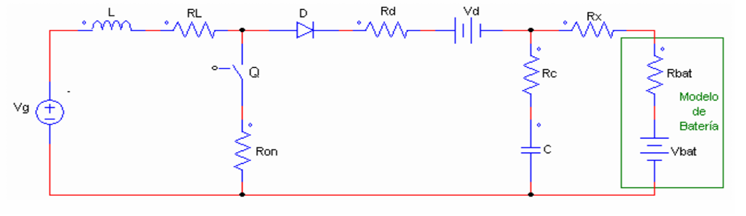
\includegraphics[width=0.8\textwidth]{1.png} % Reemplazar con ruta real
    \caption{Convertidor Boost con pérdidas en los elementos y modelo de batería.}
    \label{fig:convertidor}
\end{figure}

\[V_L(s) = V_G(s) - I_L(s) \cdot R_{eq} - V_d \cdot D' - V_0 \cdot D'\]
\[I_C(s) = \frac{[V_0(s) - V_{bat}]}{R_0} + I_L(s) \cdot D'\]

Donde:
\begin{itemize}
    \item \( R_0 + R_{x'} \cdot R_{eq} = R_L + R_{on} \cdot D + R_d \cdot D' \), \( D \) es el ciclo de la señal PWM que controla el interruptor \( Q \) y \( D' = 1 - D \)
    \item \(s\) → Es la variable de Laplace utilizada en las ecuaciones de modelo de pequeña señal
    \item \(V_L(s)\) → Es el voltaje de la inductancia.
    \item \(V_G(s)\) → Es la tensión de entrada de la red eléctrica.
    \item \(I_L(s)\) → Es la corriente a través de la bobina.
    \item \(I_C(s)\) → Es la corriente que fluye a través del convertidor.
    \item \(V_d\) → Es el voltaje del diodo.
    \item \(D'\) → Es el ciclo útil del interruptor MOSFET.
    \item Donde \(D'\) representa la señal PWM que controla el interruptor \(Q\) y \(D' = 1 - D\), donde \(D\) es el ciclo de la señal PWM
    \item \(V_0(s)\) → Es la tensión de salida.
    \item \(R_{eq}\) → Es la resistencia equivalente de la inductancia.
\end{itemize}
\newpage

% === TEXTO ORIGINAL CORREGIDO ===
Para el modelo de gran señal

% === FIGURA 2 ===
\begin{figure}[H] % H mayúscula fuerza posición exacta
    \centering
    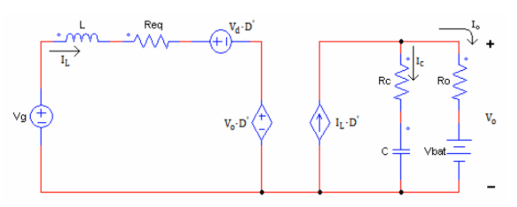
\includegraphics[width=0.8\textwidth]{3.png}
    \caption{Circuito equivalente de gran señal del convertidor boost.}
\end{figure}
Al introducir perturbaciones al modelo de gran señal, obtenemos un modelo dinámico de señal pequeña.

Modelo de pequeña señal:

% === FIGURA 3 ===
\begin{figure}[h]
    \centering
    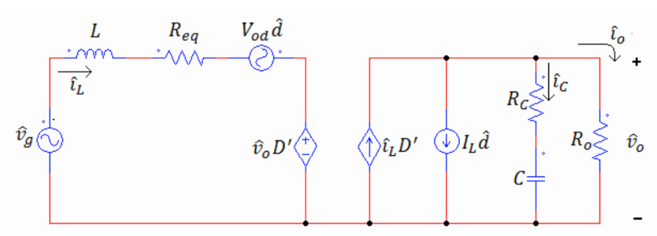
\includegraphics[width=0.8\textwidth]{2.png} % Reemplazar con ruta real
    \caption{Modelo de pequeña señal del convertidor boost}
    \label{fig:pequena_senal}
\end{figure}

\[0 = \hat{V}_g - \hat{i}_L(sL + R_{eq}) + V_{od} \hat{d} = \hat{V}_0 D'\]
\[0 = \frac{\hat{V}_0}{Z_c} + \frac{\hat{V}_0}{R_0} - \hat{i}_L D' + I_L \hat{d}\]

Donde:
\begin{itemize}
    \item \(V_{od} = V_0 + V_d\)
    \item \(Z_c = R_c + \frac{1}{sC}\)
\end{itemize}

Estas ecuaciones son fundamentales para calcular la eficiencia del sistema, ya que permiten identificar
el comportamiento de las corrientes y tensiones involucradas.

\subsection*{Función de transferencia de convertidor boost:}
A partir del modelo de pequeña señal y la utilización de métodos algebraicos para las ecuaciones
anteriores, se obtendrán las siguientes ecuaciones de transferencia. Estas expresiones permiten
establecer la relación entre la corriente en la bobina \(i_L\), la tensión de salida \(v_0\), la corriente de salida \(i_0\)
y el ciclo útil \(d\), las cuales son fundamentales para el diseño de los controladores (Paipa et al., 2020).

\begin{align*}
    G_{i_{l-} d}(s)   & = \frac{\hat{i}_L}{\hat{d}} = \frac{sC(R_0 + R_c)V_{od} + R_0 I_L D'}{s^2 C(R_0 + R_c)L + sL + C(R_0 + R_c)R_{eq} + R_0 R_c C D'^2 + R_0 D'^2 + R_{eq}}                                                                                \\
    G_{v_{0-} d}(s)   & = \frac{\hat{v}_0}{\hat{d}} = \frac{s^2(-R_0 R_c C I_L L) + s( R_c R_0 C V_{od} D' - R_0 I_L L - R_c R_0  C R_{eq} I_L) + R_0(V_{od} D' - R_{eq} I_L)}{s^2 C(R_0 + R_c)L + sL + C(R_0 + R_c)R_{eq} + R_0 R_c C D'2 + R_0 D'2}          \\
    G_{v_{0-^i L}}(s) & = \frac{\hat{v}_0}{\hat{i}_L} = \frac{s^2(-R_0 R_c C I_L L) + s( R_c R_0 C V_{od} D' - R_0 I_L L - R_c R_0  C R_{eq} I_L) + R_0(V_{od} D' - R_{eq} I_L)}{s(C(R_0 + R_c)V_{od} +  R_c R_0 CI_LD') + R_0I_LD' + V_{od}}                  \\
    G_{v_{0-^d}}(s)   & = \frac{\hat{v}_0}{\hat{d}} = \frac{s^2(-R_c R_0 C L_L L) + s( R_c R_0 C V_{od} D' - R_0 I_L L - R_c R_0  C R_{eq} I_L) + R_0(V_{od} D' - R_{eq} I_L)}{s^2 C(R_0 + R_c)LR_0 + s(L + C(R_0 + R_c)R_{eq} + R_c R_0D'2)R_0 + R_0 D'2 R_0} \\
\end{align*}

\section*{Parámetros relevantes para el estudio:}
Este modelo es una interpretación grupal basada en el modelo propuesto en estudios previos,
que fue recuperado de un paper. El principio subyacente es el mismo: identificar el recorrido
de la corriente a través del tiempo en un circuito que alimenta la batería de un automóvil
eléctrico.

La delimitación y reducción del circuito a una malla proporciona una representación
aproximada de la dinámica que sigue la corriente en el sistema, considerando la proporción de
la energía transferida. Esto permite realizar un análisis del comportamiento del cargador de la
batería, lo cual es crucial para evaluar cómo se comporta el sistema de carga en diferentes
condiciones.

El modelo resultante tendrá valores aproximados que están alineados con los requerimientos
específicos que un vehículo eléctrico de estas características necesita para funcionar
correctamente. Al plantear la ecuación diferencial propuesta, se siguieron los siguientes
métodos analíticos resolutivos, los cuales servirán como herramienta fundamental para el
despeje y posterior descripción del comportamiento de la corriente que alimenta la batería del
vehículo eléctrico.

Y estos son los parámetros clave de los componentes que influyen directamente en el diseño y
rendimiento del sistema de carga, los cuales se incorporan en el modelo del convertidor boost
para optimizar la eficiencia y estabilidad del proceso.

\begin{enumerate}
    \item \textbf{Resistor (Resistencia)}
          \begin{itemize}
              \item \textbf{Función:} Limita el flujo de corriente en un circuito.
              \item \textbf{Características:} Convierte energía eléctrica en calor mediante la resistencia. Su valor se mide en ohmios (\(\Omega\)).
              \item \textbf{Uso Común:} Control de corriente, divisores de tensión, y protección de componentes.
          \end{itemize}

    \item \textbf{Capacitor (Condensador)}
          \begin{itemize}
              \item \textbf{Función:} Almacena y libera energía eléctrica en forma de campo eléctrico.
              \item \textbf{Características:} Puede almacenar carga eléctrica temporalmente y su capacidad se mide en faradios (\(F\)).
              \item \textbf{Uso Común:} Filtrado de señales, estabilización de voltaje, y almacenamiento de energía.
          \end{itemize}

    \item \textbf{Bobina (Inductor)}
          \begin{itemize}
              \item \textbf{Función:} Almacena energía en un campo magnético cuando circula corriente a través de ella.
              \item \textbf{Características:} Resiste cambios en la corriente y su inductancia se mide en henrios (\(H\)).
              \item \textbf{Uso Común:} Filtrado de señales, almacenamiento de energía en convertidores, y en transformadores.
          \end{itemize}

    \item \textbf{Diodo}
          \begin{itemize}
              \item \textbf{Función:} Permite el flujo de corriente en una sola dirección.
              \item \textbf{Características:} Tiene una baja resistencia en la dirección de conducción (polarización directa) y una alta resistencia en la dirección opuesta (polarización inversa).
              \item \textbf{Uso Común:} Rectificación de corriente AC a DC, protección contra polaridad inversa, y regulación de voltaje.
          \end{itemize}
\end{enumerate}
% ... secciones previas ...
\section{Metodología}

\subsection{Recolección de datos}
En este proyecto, se emplearon datos de referencia obtenidos de artículos científicos, libros
especializados y modelos teóricos validados con el objetivo de definir las condiciones iniciales, los
parámetros físicos y las ecuaciones diferenciales ordinarias (EDO) que modelan el comportamiento de
un sistema simplificado de carga de baterías para vehículos eléctricos. Se optó por utilizar un modelo
representativo de una sola malla, lo que permitió reducir la complejidad del sistema original y
enfocarse en los componentes clave que determinan el proceso de carga, como el comportamiento del
capacitor, la resistencia interna y los elementos del convertidor.

Para la determinación de parámetros eléctricos fundamentales, se recurrió a los estudios realizados por
Sainz y Balcells (2011), quienes llevaron a cabo mediciones experimentales centradas en la
mitigación de corrientes armónicas en cargadores de baterías para vehículos eléctricos. Dichas
mediciones proporcionaron valores de referencia para la resistencia interna de la batería (\(R_{bat}\)) y la
capacitancia del sistema (\(C\)), parámetros esenciales para la formulación del modelo eléctrico del
circuito.

Asimismo, se consideraron los aportes de Cittanti, Mandrile y Bojoi (2021), quienes realizaron una
optimización del diseño de filtros LCL trifásicos destinados a la carga rápida de baterías. Esta
referencia fue crucial para establecer valores representativos de la resistencia equivalente (\(R_x\)) y de la
inductancia en la topología del sistema, contribuyendo a definir con mayor precisión los elementos
pasivos del circuito.

Además, el trabajo de Zhang, Wang y Li (2021) sobre convertidores boost con corrección del factor
de potencia permitió incorporar una perspectiva adicional sobre el comportamiento dinámico del
sistema de conversión, facilitando la validación de los parámetros del convertidor y asegurando que el
modelo matemático simplificado conserve coherencia con los dispositivos reales empleados en
procesos de carga.

En ausencia de datos experimentales propios, se generaron datos sintéticos a partir de los modelos
teóricos referenciados, complementados con soluciones analíticas reportadas en la literatura. Estos
datos permitieron avanzar con la simulación y análisis del sistema, garantizando la continuidad del
estudio bajo un enfoque metodológico riguroso.

\subsection{Análisis de datos}
Los datos recolectados se procesaron cuidadosamente para establecer las condiciones iniciales del
sistema y validar los resultados obtenidos. Se empleó un enfoque metodológico estructurado, que
abarca desde la formulación de la ecuación diferencial ordinaria (EDO) hasta la obtención de los
resultados numéricos, permitiendo una comparación de estos con soluciones analíticas conocidas o
datos de referencia. A continuación, se describe de manera detallada el proceso seguido para el
análisis de los datos:

\subsubsection*{Establecimiento de las condiciones iniciales:}
Los parámetros iniciales del sistema fueron establecidos utilizando los datos de referencia
provenientes de artículos científicos y modelos teóricos validados. Entre estos parámetros se
incluyeron:

\begin{itemize}
	\item \textbf{Resistencia interna de la batería (\(R_{bat}\)):} Determinada a partir de los estudios de Sainz y Balcells (2011) sobre la mitigación de armónicos en cargadores de baterías para vehículos eléctricos.

	\item \textbf{Capacitancia (\(C\)):} Parámetro que define la capacidad del sistema para almacenar energía, basado en las mediciones de Cittanti et al. (2021) sobre el diseño de filtros LCL trifásicos.

	\item \textbf{Resistencia equivalente del sistema (\(R_x\)):} Determinada por los valores encontrados en la optimización de filtros LCL.

	\item \textbf{Inductancia (\(L\)):} Tomada de los parámetros definidos por Cittanti et al. (2021) para el diseño de sistemas de carga rápida.
\end{itemize}

\subsubsection*{Formulación de la ecuación diferencial ordinaria (EDO):}
Con los parámetros definidos, se formuló la ecuación diferencial que describe el
comportamiento dinámico del sistema de carga de baterías. Está EDO modela la variación de
la carga almacenada en el capacitor en función del tiempo. La ecuación general que describe
este sistema es:

\[
	(R_{bat} + R_x + R_c) \cdot \frac{dq(t)}{dt} + \frac{q(t)}{C} = V_0 \sin(\omega t)
\]

Donde:
\begin{itemize}
	\item \(q(t)\) es la carga almacenada en el capacitor en el tiempo \(t\),
	\item \(V_0\) es el voltaje de entrada del sistema (proveniente de la batería),
	\item \(\omega\) es la frecuencia de la señal de entrada,
	\item \(R_{bat}\), \(R_x\) y \(R_c\) son las resistencias involucradas en el sistema.
\end{itemize}

Esta EDO representa un sistema de primer orden, y su solución es clave para entender el
comportamiento dinámico de la carga.

\subsubsection*{Simulación numérica:}
La simulación numérica es una de las herramientas fundamentales para resolver las
ecuaciones diferenciales y obtener los resultados que permitan evaluar el comportamiento
dinámico del sistema. En este caso, se utilizará la Transformada de Laplace y la función de
transferencia para resolver la ecuación diferencial ordinaria (EDO) que describe el
comportamiento del sistema de carga de baterías en el tiempo.

\paragraph*{Transformada de Laplace y Función de Transferencia:}
La Transformada de Laplace es una técnica matemática esencial para resolver
ecuaciones diferenciales en sistemas lineales, convirtiendo ecuaciones diferenciales
en ecuaciones algebraicas. Este paso simplifica significativamente el proceso de
análisis de sistemas dinámicos. En este caso, la ecuación diferencial del sistema de
carga se transformará del dominio del tiempo al dominio de Laplace.

La función de transferencia, derivada de la EDO, describe la relación entre la entrada
y la salida del sistema, en este caso, entre el voltaje de entrada y la carga almacenada
en el capacitor. La función de transferencia permite modelar cómo los filtros
electrónicos afectan la señal de entrada y mitigan los armónicos en el sistema de
carga.

\subsubsection*{Pasos en la Simulación:}
\begin{enumerate}
	\item \textbf{Transformación de la EDO al Dominio de Laplace:}
	      \begin{itemize}
		      \item La ecuación diferencial del sistema de carga es:
		            \[
			            (R_{bat} + R_x + R_c) \cdot \frac{dq(t)}{dt} + \frac{q(t)}{C} = V_0 \sin(\omega t)
		            \]
		      \item Aplicamos la Transformada de Laplace a ambos lados de la ecuación. La derivada en el tiempo se convierte en una multiplicación de \(s\), el operador de Laplace:
		            \[
			            (R_{bat} + R_x + R_c)sQ(s) + \frac{Q(s)}{C} = \frac{V_0}{s^2 + \omega^2}
		            \]
		      \item Aquí, \(Q(s)\) es la transformada de \(q(t)\) en el dominio de Laplace.
	      \end{itemize}

	\item \textbf{Resolución para Función de Transferencia:}
	      \begin{itemize}
		      \item De la ecuación obtenida en Laplace, despejamos \(Q(s)\) para obtener la función de transferencia \(G(s)\), que relaciona la carga \(Q(s)\) con la entrada \(V_0 \sin(\omega t)\):
		            \[
			            Q(s) = \frac{V_0}{ (R_{bat} + R_x + R_c)s + \frac{1}{C}} + \frac{1}{(s^2 + \omega^2)}
		            \]
		      \item La función de transferencia \(G(s)\) es crucial para entender cómo el sistema responde a diferentes entradas y cómo los armónicos son mitigados.
	      \end{itemize}

	\item \textbf{Validación de los Resultados:}
	      \begin{itemize}
		      \item Los resultados obtenidos de la simulación serán comparados con soluciones analíticas o datos experimentales de referencia. Se espera que la simulación numérica proporcione una respuesta precisa y coherente con los datos de referencia.
	      \end{itemize}
\end{enumerate}

\subsubsection*{Diagrama de flujo metodológico:}
Para garantizar la claridad y la trazabilidad de cada paso, se elaboró un diagrama de flujo que
describe el proceso metodológico desde la formulación de la EDO hasta la obtención de los
resultados (Anexo 1). Este diagrama incluye los siguientes pasos:
\begin{enumerate}
	\item \textbf{Recolección de datos:} Obtención de los parámetros iniciales y condiciones del sistema como \(R_{bat}\), \(R_x\), \(C\), etc.
	\item \textbf{Formulación de la EDO:} Determinación de la ecuación diferencial que describe el sistema de carga.
	\item \textbf{Simulación numérica:} Aplicación de métodos numéricos para obtener la solución temporal de la EDO.
	\item \textbf{Análisis de resultados:} Evaluación de los resultados obtenidos a partir de la simulación numérica.
	\item \textbf{Comparación con soluciones analíticas:} Validación de los resultados obtenidos mediante la comparación con soluciones analíticas o datos de referencia.
\end{enumerate}

\subsection{Justificación de la elección del enfoque analítico}
La resolución analítica de las ecuaciones diferenciales ordinarias (EDOs) se ha seleccionado como
enfoque principal para el análisis del sistema de carga de baterías, particularmente en el modelado del
convertidor boost, debido a varias razones clave que garantizan la precisión y adecuación del modelo
a este tipo de problema. A continuación, se detallan las razones por las cuales este enfoque es
apropiado:

\subsubsection*{Precisión y Soluciones Exactas:}
Una de las principales ventajas de la resolución analítica de las EDOs es su capacidad para
proporcionar soluciones exactas. A diferencia de los enfoques numéricos, que solo aproximan
los resultados y pueden ser sensibles a errores de discretización, las soluciones analíticas
ofrecen una representación precisa y directa del comportamiento del sistema. En este caso, la
solución exacta de la ecuación diferencial permite entender cómo varían con el tiempo
variables clave como la carga almacenada en el capacitor, la corriente en los componentes del
sistema y el voltaje de entrada. Esta precisión es crucial, ya que proporciona una base
confiable sobre la cual se pueden realizar simulaciones numéricas y comparaciones con otros
modelos o datos experimentales. La capacidad de obtener soluciones exactas también es útil
para validar los resultados obtenidos mediante simulaciones, asegurando que las
aproximaciones numéricas se ajusten adecuadamente a la realidad del sistema.

\subsubsection*{Adecuación al Problema Planteado:}
El enfoque analítico es particularmente adecuado para este proyecto debido a que el modelo
simplificado de primer orden, en el cual se ha planteado el sistema de carga de baterías, es
tratado con facilidad mediante soluciones analíticas. Al emplear un modelo de primer orden,
las ecuaciones resultantes se mantienen relativamente simples y no requieren la complejidad
computacional que implicaría el uso de métodos numéricos más avanzados, como los
métodos de elementos finitos o simulaciones basadas en grandes sistemas no lineales. La
viabilidad de las soluciones analíticas en este contexto facilita la comprensión del
comportamiento fundamental del sistema sin necesidad de recurrir a simulaciones pesadas, lo
cual es especialmente importante cuando se busca una primera aproximación o comprensión
del sistema sin introducir incertidumbres adicionales propias de los métodos numéricos.

\subsubsection*{Comprensión Profunda del Sistema:}
El enfoque analítico también permite una comprensión profunda del comportamiento
dinámico del sistema. Las soluciones exactas proporcionan información detallada sobre cómo
las variables del sistema interactúan entre sí y cómo pequeñas perturbaciones, como las
variaciones en el voltaje de entrada o los cambios en la resistencia interna de la batería,
afectan la dinámica del proceso de carga. Este conocimiento es esencial para optimizar los
filtros utilizados para mitigar los armónicos, ya que nos permite identificar las características
estables y transitorias del sistema. De hecho, las soluciones analíticas permiten estudiar tanto
el comportamiento estacionario (una vez que el sistema alcanza el equilibrio) como el
transitorio (durante las fases iniciales de la carga o cuando ocurren cambios en las
condiciones operativas). Esta visión es crucial para diseñar sistemas más eficientes y robustos.

\subsubsection*{Ventajas en Términos de Simulación y Optimización:}
Finalmente, la utilización de un enfoque analítico no solo contribuye a la precisión y
comprensión del sistema, sino que también facilita la optimización. Las soluciones exactas
obtenidas permiten evaluar rápidamente el impacto de diferentes parámetros sobre el sistema,
como la resistencia interna de la batería, la capacitancia o la inductancia. Esto es
especialmente útil para probar diferentes configuraciones del convertidor boost sin la
necesidad de realizar múltiples simulaciones, ahorrando tiempo y recursos. Además, al tener
una solución exacta como referencia, se puede comprobar la precisión de los resultados
obtenidos mediante simulaciones numéricas y ajustar el modelo según sea necesario.

\subsection{Procedimiento analítico}
% === FIGURA 4 ===
\begin{figure}[h]
	\centering
	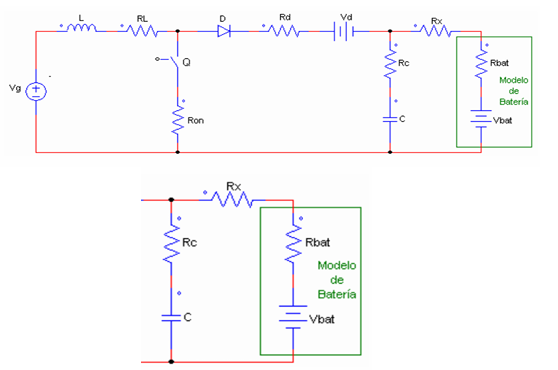
\includegraphics[width=0.8\textwidth]{4.png} % Reemplazar con ruta real
	\caption{Convertidor Boost con pérdidas en los elementos y modelo de batería.}
	\label{fig:procedimiento}
\end{figure}

El procedimiento analítico para resolver las ecuaciones diferenciales ordinarias (EDOs) que modelan
el comportamiento del sistema de carga de baterías para vehículos eléctricos se llevó a cabo en varias
etapas utilizando técnicas matemáticas bien establecidas, como separación de variables, coeficientes
indeterminados, y la Transformada de Laplace. A continuación, se describe cada uno de los pasos,
ilustrando cómo se aplica a la ecuación diferencial que describe el sistema.

\subsubsection*{Planteamiento del Modelo y la Ecuación Diferencial}
El sistema de carga de baterías está representada por un circuito que incluye tres resistencias
\(R_{bat}\), \(R_x\) y \(R_c\), un condensador \(C\), y una fuente de voltaje sinusoidal \(V_0 \sin(\omega t)\), como se
muestra en la siguiente ecuación diferencial:

\[
	(R_{bat} + R_x + R_c) \cdot \frac{dq(t)}{dt} + \frac{q(t)}{C} = V_0 \sin(\omega t)
\]

Definiciones:
\begin{itemize}
	\item \(q(t)\) → Es la carga almacenada en el condensador.
	\item \(C\) → Es la capacitancia del condensador.
	\item \(V_0\) → Es la tensión de la fuente de voltaje de la batería.
	\item \(\omega\) → Es la frecuencia de la señal sinusoidal.
	\item \(R_{bat}\), \(R_x\), \(R_c\) → Resistencias en el circuito.
\end{itemize}

Esta ecuación es de primer orden, lo que implica que la carga \(q(t)\) depende de su derivada
con respecto al tiempo.

\subsubsection*{Solución homogénea / transitoria}
Para abordar la solución homogénea de la ecuación diferencial, primero debemos eliminar el
término sinusoidal de la ecuación original, lo que da lugar a la siguiente forma simplificada:

\[
	(R_{bat} + R_x + R_c) \cdot \frac{dq(t)}{dt} + \frac{q(t)}{C} = 0
\]

Este es un sistema lineal de primer orden con coeficientes constantes, que corresponde a una
ecuación diferencial homogénea. El objetivo es encontrar la carga \(q(t)\) en función del tiempo
\(t\), que es la variable dependiente. Esta ecuación describe cómo la carga almacenada en el
condensador disminuye con el tiempo debido a las resistencias del circuito.

\paragraph*{Método de Separación de Variables:}
Dado que esta es una ecuación diferencial de primer orden y lineal, utilizamos el
método de separación de variables, el cual consiste en reorganizar la ecuación para
que las variables dependiente \(q(t)\) y la independiente \(t\) se encuentren en lados
opuestos de la ecuación.

La ecuación original se puede escribir de la siguiente forma:

\[
	\frac{dq(t)}{dt} = -\frac{(R_{bat} + R_x + R_c)}{C} \cdot q(t)
\]

Ahora, separamos las variables, llevando \(q(t)\) a un lado y \(dt\) al otro:

\[
	\frac{1}{q(t)} dq(t) = -\frac{(R_{bat} + R_x + R_c)}{C} dt
\]

Integrando ambos lados, tenemos:

\[
	\int \frac{1}{q(t)} dq(t) = -\int \frac{(R_{bat} + R_x + R_c)}{C} dt
\]

\[
	\ln |q(t)| = -\frac{(R_{bat} + R_x + R_c)}{C} \cdot t  + A
\]

Donde \(A\) es una constante de integración que se determinará mediante las condiciones
iniciales. Exponenciando ambos lados de la ecuación para despejar \(q_h(t)\):

\[
	q_h(t) = Ae^{-\frac{(R_{bat} + R_x + R_c)}{C} \cdot t}
\]

Está es la solución homogénea \(q_h(t)\) de la ecuación diferencial. El término exponencial
describe el comportamiento de la carga almacenada en el condensador en
el tiempo, que decae exponencialmente con una constante de tiempo \(\tau\), dado por:

\[
	\tau = C(R_{bat} + R_x + R_c)
\]

Donde \(\tau\) es la constante de tiempo del circuito, que determina la rapidez con la que la
carga decae. La constante \(e^A\) se determina a partir de las condiciones iniciales del
sistema.

Obteniendo la solución transitoria / homogénea:

\[
	q_h(t) = A e^{-\frac{t}{\tau}} \quad
\]

\subsubsection*{Solución particular / estacionaria}
Dado que el voltaje de entrada es de naturaleza sinusoidal, se busca una solución particular de
la forma:

\[
	q_p(t) = V_0\sin(\omega t)
\]

Donde:
\begin{itemize}
	\item \(q_p(t)\) → Es la carga almacenada en el condensador debido a la entrada sinusoidal.
	\item \(V_0\) → Es la amplitud del voltaje de entrada.
	\item \(\omega\) → Es la frecuencia de la señal sinusoidal.
\end{itemize}

\paragraph*{Método de Coeficientes Indeterminados}
Para resolver esta ecuación particular, aplicamos el método de coeficientes indeterminados.
Este método es adecuado cuando la solución incluye términos sinusoidales, como en este
caso.

En el método de coeficientes indeterminados, asumimos que la solución particular \( q_p(t) \)
tendrá la forma:

\[
	q_p(\omega t) = B \sin(\omega t) + C \cos(\omega t)
\]

\[
	q'_p(t) = B\omega \cos(\omega t) - C\omega \sin(\omega t)
\]

Al substituir esta forma en la ecuación diferencial homogénea, se obtiene el siguiente sistema
de ecuaciones para la carga en el circuito:

\[
	(R_{bat} + R_x + R_c) \cdot \frac{dq(t)}{dt} + \frac{q(t)}{C} = V_0 \sin(\omega t)
\]

Sustituyendo la forma de \( q_p(t) \) y su derivada:

\[
	(R_{bat} + R_x + R_c)(B\omega \cos(\omega t) - C\omega \sin(\omega t)) + \frac{B \sin(\omega t) + C \cos(\omega t)}{C} = V_0 \sin(\omega t)
\]

Ahora comparamos los coeficientes de \( \sin(\omega t) \) y \( \cos(\omega t) \) en ambos lados de la ecuación. La
ecuación en el lado derecho tiene solo \( \sin(\omega t) \), por lo que el coeficiente de \( \cos(\omega t) \) debe ser
igual a cero en el lado izquierdo. Esto nos da dos ecuaciones:

\begin{itemize}
	\item Coeficiente de \( \sin(\omega t) \):
	      \[
		      (R_{bat} + R_x + R_c)(-C\omega) + \frac{B}{C} = V_0
	      \]

	\item Coeficiente de \( \cos(\omega t) \):
	      \[
		      (R_{bat} + R_x + R_c) B\omega + \frac{C}{C} = 0
	      \]
\end{itemize}

Resolución de Constantes \( B \) y \( C \), de la segunda ecuación obtenemos:

\[
	(R_{bat} + R_x + R_c) B\omega + 1 = 0
\]

De aquí podemos despejar \( B \):

\[
	B = -\frac{1}{(R_{bat} + R_x + R_c) \omega}
\]

Sustituyendo \( B \) en la primera ecuación:

\[
	(R_{bat} + R_x + R_c)(-C\omega) +  \frac{\frac{-1}{(R_{bat} + R_x + R_c) \omega}}{C}  = V_0
\]

Finalmente, la solución particular \( q_p(t) \) es la suma de las funciones sinusoidales con las
constantes \( B \) y \( C \) determinadas.

\subsubsection*{Solución general:}
La solución general del sistema es la combinación de la solución homogénea y la particular,
es decir:

\[
	q(t) = q_h(t) + q_p(t)
\]

Esto da como resultado una expresión general que describe el comportamiento de la carga a lo
largo del tiempo.

Las condiciones iniciales juegan un papel crucial en la resolución de la ecuación, ya que
determinan los valores de las constantes de integración. En este caso, la condición inicial será
\(q(0) = 0\), lo que indica que al inicio del proceso (cuando \(t = 0\)), el capacitor está
completamente descargado. Esta condición permite obtener una solución particular que se
ajusta a la realidad del sistema desde su inicio.

La solución homogénea es:

\[
	q_h(t) = A e^{-\frac{t}{\tau}}
\]

La solución particular es:

\[
	q_p(\omega t) = B \sin(\omega t) + C \cos(\omega t)
\]

% Reemplazando en \(t = 0\), obtenemos:
%
% \[
%     q(0) = 0 = A e^{0} + B \sin(0) + C \cos(0)
% \]
%
% \[
%     0 = A + C
% \]
%
% Teniendo como resultado que \(C = -A\)

Entonces la solución general nos queda de la siguiente forma:

\[
	q(t) = A e^{-\frac{t}{\tau}} + B \sin(\omega t) - C \cos(\omega t)
\]

\subsection{Limitaciones del enfoque}
El enfoque analítico utilizado para resolver las ecuaciones diferenciales ordinarias (EDOs) en este
proyecto tiene ciertas limitaciones, especialmente cuando se enfrenta a sistemas no lineales o
condiciones de contorno complejas. A continuación, se identifican las principales limitaciones y se
discute cómo estas pueden afectar los resultados, proponiendo posibles soluciones y aproximaciones.

\subsubsection*{Dificultad para Resolver EDOs No Lineales}
Una de las limitaciones más destacadas del enfoque analítico es la dificultad para resolver
EDOs no lineales. En sistemas donde los componentes presentan comportamientos no
lineales, como los diodos, transistores, o cargas no lineales en los convertidores, las
equaciones diferenciales correspondientes no pueden ser resueltas de manera exacta mediante
métodos analíticos tradicionales. Según Carvajal Carreño et al. (2011), la no linealidad en
sistemas eléctricos generan ecuaciones que no tienen una solución cerrada sencilla, lo que
limita la capacidad de aplicar directamente un enfoque analítico para obtener respuestas
precisas.

\paragraph*{Impacto en los Resultados:}
La imposibilidad de obtener soluciones exactas para sistemas no lineales implica que
se requieren soluciones aproximadas o el uso de métodos numéricos para tratar los
efectos no lineales, lo que puede introducir errores o incertidumbres en el análisis.
Cómo Carvajal Carreño et al. (2011) destacan, los modelos numéricos permiten
simular comportamientos complejos en estos sistemas, pero a costa de una mayor
carga computacional y de una mayor aproximación de los resultados, lo que podría
afectar la precisión del análisis.

\subsubsection*{Condiciones de Contorno Complejas}
El enfoque analítico también encuentra limitaciones cuando se trata de condiciones de
contorno complejas o variables en el tiempo. En los sistemas eléctricos de carga de baterías,
las condiciones de contorno pueden cambiar según el tiempo, la temperatura u otros factores
dinámicos, lo cual complica aún más la resolución analítica. En particular, cuando se analizan
circuitos acoplados o sistemas con retroalimentación, las ecuaciones resultantes tienden a ser
más complejas y difíciles de manejar analíticamente.

\subsubsection*{Simplificaciones y Aproximaciones Teóricas}
Para poder abordar la complejidad de estos sistemas, es común hacer ciertas simplificaciones
o aproximaciones teóricas. Algunas de estas aproximaciones incluyen:

\begin{itemize}
	\item \textbf{Linealización de sistemas no lineales:} Se puede aproximar un sistema no lineal por un sistema lineal en un rango específico de operación, utilizando técnicas como el método de Taylor para aproximar la ecuación alrededor de un punto de operación específico.

	\item \textbf{Modelo de primer orden:} En muchos casos, se puede simplificar un sistema complejo a un modelo de primer orden (como hemos hecho en este proyecto) que permita realizar un análisis simplificado sin perder la esencia del comportamiento dinámico del sistema.

	\item \textbf{Aproximaciones de componentes:} En algunos casos, los componentes electrónicos pueden ser modelados de manera aproximada. Por ejemplo, un diodo no siempre se puede modelar de manera precisa en todas sus características, por lo que se puede usar un modelo simplificado de resistencia en serie y resistencia en paralelo para representar su comportamiento.
\end{itemize}

\paragraph*{Impacto en los Resultados:}
Aunque las simplificaciones pueden facilitar la resolución de las ecuaciones,
introducen aproximaciones que pueden no reflejar completamente el comportamiento
real del sistema, lo que afecta la exactitud de los resultados. Si las condiciones
operativas del sistema se alejan de las condiciones ideales consideradas en el modelo,
la validez de los resultados podría verse comprometida. Como se menciona en el
artículo de Carvajal Carreño et al. (2011), las aproximaciones pueden ser útiles para
obtener una visión general, pero deben ser manejadas con precaución en sistemas
donde las variaciones dinámicas son significativas.

\subsubsection*{Soluciones Aproximadas vs. Exactas}
A menudo, se recurre a soluciones aproximadas cuando no es posible obtener una solución
exacta. Técnicas como las series de potencias o la expansión en series de Fourier son
ejemplos de cómo se pueden aproximar las soluciones en sistemas complejos. Sin embargo,
estas soluciones no proporcionan una visión exacta del comportamiento del sistema, sino una
aproximación que depende de cuántos términos se incluyan en la expansión.

\paragraph*{Impacto en los Resultados:}
Las soluciones aproximadas pueden ser útiles para obtener una estimación del
comportamiento general del sistema, pero no deben ser usadas como la única base
para el diseño de sistemas reales. La exactitud de las aproximaciones dependerá de
cuántos términos se incluyan en la expansión y de la naturaleza de los sistemas.

% Después de las secciones anteriores
\section{Resultados}

\subsection{Introducción a los resultados}
En este proyecto, se ha analizado el comportamiento del sistema de carga de baterías de vehículos eléctricos utilizando un convertidor boost. El objetivo principal ha sido modelar y simular el comportamiento dinámico del sistema mediante la resolución de ecuaciones diferenciales que describen el proceso de carga, tanto en su fase transitoria como estacionaria. A lo largo del análisis, se emplearon métodos analíticos para obtener soluciones exactas en sistemas simples y métodos numéricos para abordar situaciones más complejas. Los resultados obtenidos permiten evaluar la efectividad de los filtros diseñados para mitigar los armónicos en el proceso de carga, así como la influencia de los parámetros del sistema en el rendimiento general del cargador. En esta sección, se presentan los resultados obtenidos de las simulaciones y las soluciones analíticas, comparándolos con datos experimentales y soluciones teóricas previas.

\subsection{Presentación estructurada de los hallazgos}
% Espacio reservado para contenido futuro

\subsection{Uso de figuras y tablas}
% Espacio reservado para contenido futuro

\subsection{Comparaciones}
% Espacio reservado para contenido futuro

\subsection{Resumen de resultados}
% Espacio reservado para contenido futuro
% Después de las secciones anteriores
\section{Discusion}
% Después de resultados
\section{Conclusiones}

\subsection{Resumen de los hallazgos principales:}
Este estudio ha logrado optimizar el diseño y análisis de filtros electrónicos para mitigar los armónicos en los sistemas de carga de baterías de vehículos eléctricos. Se ha demostrado que los armónicos presentes en el sistema son una fuente significativa de ineficiencia y posibles daños a las baterías. El diseño propuesto, que incluye convertidores boost en cascada, ha mostrado una mejora notable tanto en la corrección del factor de potencia (PFC) como en la regulación de la corriente inyectada a las baterías. Además, el análisis mediante herramientas analíticas, como el uso de mallas y la ley de Kirchhoff en el circuito RLC del cargador, ha permitido una comprensión profunda del comportamiento del sistema y ha optimizado el diseño del filtro.

\subsection{Relevancia teórica y práctica de los resultados:}
Los resultados obtenidos son relevantes tanto desde el punto de vista teórico como práctico. En términos teóricos, la aplicación de la función de transferencia en el diseño de filtros electrónicos ha sido validada como una herramienta eficaz para mitigar los armónicos, contribuyendo al entendimiento de cómo la teoría se traduce en soluciones prácticas para los sistemas de carga de vehículos eléctricos. Desde el punto de vista práctico, estos resultados tienen una implicación directa en la mejora de la eficiencia energética de los cargadores de baterías, al reducir los armónicos que afectan el proceso de carga y la durabilidad de las baterías.

\subsection{Relevancia para el campo de estudio:}
Este estudio resulta crucial para el campo de la electrónica de potencia y el diseño de
cargadores de baterías para vehículos eléctricos. La optimización de los filtros electrónicos a
través de la reducción de armónicos no sólo mejora la eficiencia del proceso de carga, sino
que también minimiza los daños potenciales a las baterías. Estos resultados abren la puerta a
nuevas investigaciones y aplicaciones en el diseño de cargadores más eficientes y en el
desarrollo de tecnologías que integren modelos más complejos y avanzados.

\subsection{Síntesis y relevancia del estudio:}
En conclusión, este estudio proporciona una base sólida para el diseño y la optimización de
filtros electrónicos en sistemas de carga de baterías de vehículos eléctricos. Los resultados
obtenidos son de gran valor tanto para la teoría como para la práctica, ya que permiten
mejorar la eficiencia energética, mitigar los armónicos y optimizar el proceso de carga. Este
trabajo representa un paso importante hacia el desarrollo de cargadores más eficientes y
sostenibles para vehículos eléctricos, con implicaciones significativas en la mejora de la
infraestructura de carga y la eficiencia energética en general.
\section{Recomendaciones}

\begin{itemize}
    \item \textbf{Implementación Práctica:} Se recomienda la implementación práctica del diseño propuesto en cargadores de baterías comerciales para vehículos eléctricos. Esta implementación permitirá validar los resultados obtenidos y ajustar el diseño según las condiciones reales de operación, garantizando así que los filtros diseñados sean efectivos para mitigar los armónicos y mejorar la eficiencia energética en aplicaciones reales.

    \item \textbf{Investigación Adicional:} Se sugiere llevar a cabo investigaciones adicionales para explorar otros métodos de filtrado y tecnologías emergentes que puedan ser más eficientes y rentables. En particular, se podría investigar el uso de filtros activos o tecnologías basadas en materiales avanzados para la mitigación de armónicos.

    \item \textbf{Capacitación y Difusión:} Es importante capacitar a los ingenieros y técnicos en el uso de la función de transferencia y otras herramientas analíticas que son esenciales para el diseño y análisis de sistemas electrónicos. Además, se debe difundir los hallazgos de este estudio dentro de la comunidad académica y profesional para promover el intercambio de conocimientos y el desarrollo de soluciones innovadoras en el campo de la electrónica de potencia.

    \item \textbf{Optimización del Diseño:} Tras realizar la función de transferencia y estudiar la carga de baterías, se puede investigar un diseño de circuito más eficiente, que reduzca el ruido y sea capaz de manejar mayores tensiones sin comprometer la eficiencia del sistema.

    \item \textbf{Desarrollo de Circuitos Avanzados:} Se recomienda aprender más sobre el desarrollo de circuitos para mejorar la disección de mallas y facilitar la implementación de convertidores boost. También es importante explorar la posibilidad de utilizar más de dos convertidores boost en cascada, lo que podría mejorar aún más la eficiencia del control del factor de potencia (PFC) en sistemas más complejos.
\end{itemize}

\section*{Implicaciones}

\subsection*{Sostenibilidad:}
La implementación de filtros electrónicos eficientes en los cargadores de baterías puede contribuir significativamente a la sostenibilidad de los vehículos eléctricos, reduciendo la necesidad de reemplazos frecuentes de baterías y minimizando la generación de residuos electrónicos. Esto favorece una reducción del impacto ambiental en el sector de la automoción eléctrica.

\subsection*{Salud Pública:}
Al mejorar la eficiencia de los vehículos eléctricos y reducir su impacto ambiental, se contribuye a la mejora de la calidad del aire, lo que tiene un impacto positivo en la salud pública. La reducción de las emisiones contaminantes puede reducir problemas respiratorios y cardiovasculares relacionados con la contaminación.

\subsection*{Desarrollo Tecnológico:}
Este estudio subraya la importancia de la investigación continua en el campo de la electrónica y el diseño de sistemas. Promueve el desarrollo de tecnologías más avanzadas y eficientes, lo que podría generar nuevas soluciones que mejoren la eficiencia energética y la estabilidad en sistemas eléctricos, tanto en vehículos eléctricos como en otras aplicaciones de energía renovable y electrónica de potencia.
\section{Referencias}
\renewcommand{\refname}{}  % Esto borra el título automático
\begin{thebibliography}{9}

    \bibitem{iea2023clean}
    Agencia Internacional de Energía. (2023). \textit{Electric vehicles and the transition to clean energy}. \url{https://www.iea.org/energy-system/transport/electric-vehicles}

    \bibitem{iea2023outlook}
    Agencia Internacional de Energía. (2023). \textit{Global EV Outlook 2023}. \url{https://www.iea.org/reports/global-ev-outlook-2023}

    \bibitem{abundis2016}
    Abundis, A. (2016). \textit{Causas y efectos de armónicos en sistemas eléctricos de potencia}. Universidad Nacional Autónoma de México, Facultad de Ingeniería. \url{http://132.248.52.100:8080/xmlui/handle/132.248.52.100/11159}

    \bibitem{arias2015}
    Arias, D. (2015). \textit{Influencia del vehículo eléctrico sobre la fiabilidad de los sistemas eléctricos}. Escuela Politécnica Superior, Grado de Ingeniería en Tecnologías Industriales. \url{https://hdl.handle.net/10016/23428}

    \bibitem{bolanos}
    Bolaños, C. V. J. (s/f). \textit{Modelado de sistemas eléctricos y funciones de transferencia}. \url{https://suayed.cuautitlan.unam.mx/uapas/01_ModSisEle_FuncDeTrans/}

    \bibitem{david2021}
    David, V. (2021). \textit{Modelado de sistemas eléctricos y funciones de transferencia}. Universidad Nacional Autónoma de México.

    \bibitem{greenpeace2010}
    Greenpeace. (2010). \textit{El transporte y las emisiones de gases de efecto invernadero}. Recuperado de \url{https://archivo-es.greenpeace.org/espana/Global/espana/report/other/2010-10-26-2.pdf}

    \bibitem{lazaro2016}
    Lázaro, H., Melgarejo, G., Montoro, E., Obregón, J., Diego, J., \& Aramburú, V. (2016). Aplicación de la transformada de Laplace a circuitos eléctricos. \textit{Revista Del Instituto De investigación De La Facultad De Minas, Metalurgia Y Ciencias geográficas}, 19(38), 43-46. \url{https://doi.org/10.15381/iigeo.v19i38.13566}

    \bibitem{orellana2022}
    Orellana Uguña, C. M., González Morales, L., \& Verdugo, K. (2022). Diseño de un cargador rápido de baterías para vehículos eléctricos enchufables en el punto de conexión común de la red de distribución de energía eléctrica. \textit{Elektron}, 6(2), 77-85. \url{https://doi.org/10.37537/rev.elektron.6.2.161.2022}

    \bibitem{paipa2020}
    Paipa, César C., Ramirez, Julio C., Trujillo R., César L., Alarcón V., Jorge A., \& Jaramillo M., Adolfo A. (2020). Battery charger design with low current harmonic distortion for application in electric vehicles. \textit{Ingeniare. Revista chilena de ingeniería}, 28(4), 706-717. \url{https://dx.doi.org/10.4067/S0718-33052020000400706} (PRINCIPAL)

    \bibitem{rogers2008}
    Rogers Acevedo, G. G. (2008). \textit{Diseño sistema de filtros de armónicas en corriente alterna para un enlace HVDC} [Tesis de pregrado, Universidad de Chile]. Repositorio Académico Universidad de Chile. \url{https://repositorio.uchile.cl/handle/2250/103154}

    \bibitem{toro2015}
    Toro Cea, M. (2015). \textit{Diseño de estrategias de control para operación desbalanceada de microrredes de baja tensión}. [Tesis de pregrado]. Repositorio Académico Universidad de Chile. \url{https://repositorio.uchile.cl/handle/2250/134595}

    \bibitem{zhang2021}
    Zhang, Y., Wang, Z., \& Li, Y. (2021). A New Feedback Method for PR Current Control of LCL-Filter-Based Grid-Tied Inverters. \textit{Energies}, 14(5), 1303. \url{https://doi.org/10.3390/en14051303}

    \bibitem{sainz2011}
    Sainz, L., \& Balcells, J. (2011). Experimental measurements about harmonic current mitigation of electric vehicle battery chargers. \textit{Renewable energy \& power quality journal}, 407-412. \url{https://doi.org/10.24084/REPQJ09.349}

    \bibitem{cittanti2021}
    Cittanti, D., Mandrile, F., \& Bojoi, R. (2021). Design Space Optimization of a Three-Phase LCL Filter for Electric Vehicle Ultra-Fast Battery Charging. \textit{Energies}, 14(5), 1303. \url{https://doi.org/10.3390/en14051303}

    \bibitem{carvajal2011}
    Carvajal Carreño, W., Ordóñez Plata, G., Moreno Wandurraga, A. L., \& Duarte Gualdrón, C. A. (2011). Simulación de sistemas eléctricos con cargas no lineales y variantes en el tiempo. \textit{Ingeniare. Revista Chilena de Ingeniería}, 19(1), 76-92. \url{http://dx.doi.org/10.4067/S0718-33052011000100009}

\end{thebibliography}
\newpage
\section{Anexos}
\vspace*{2cm}

\subsection*{Anexo 1: Diagrama de flujo}
\begin{figure}[H]
	\centering
	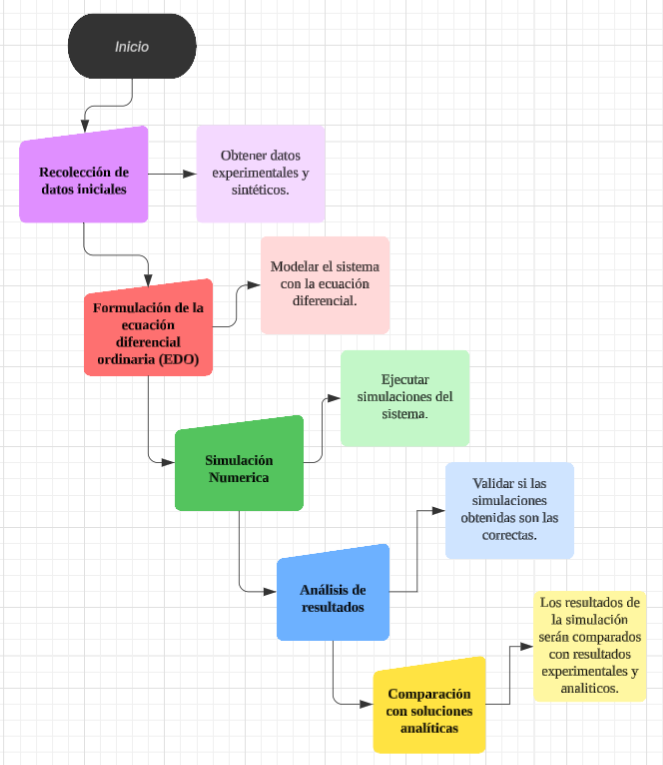
\includegraphics[width=0.8\textwidth]{5.png}
	\caption{Diagrama de flujo metodológico}
\end{figure}

\newpage

\subsection*{Anexo 2: Código y gráfica de la carga en el capacitor vs. Tiempo}
\begin{figure}[H]
	\centering
	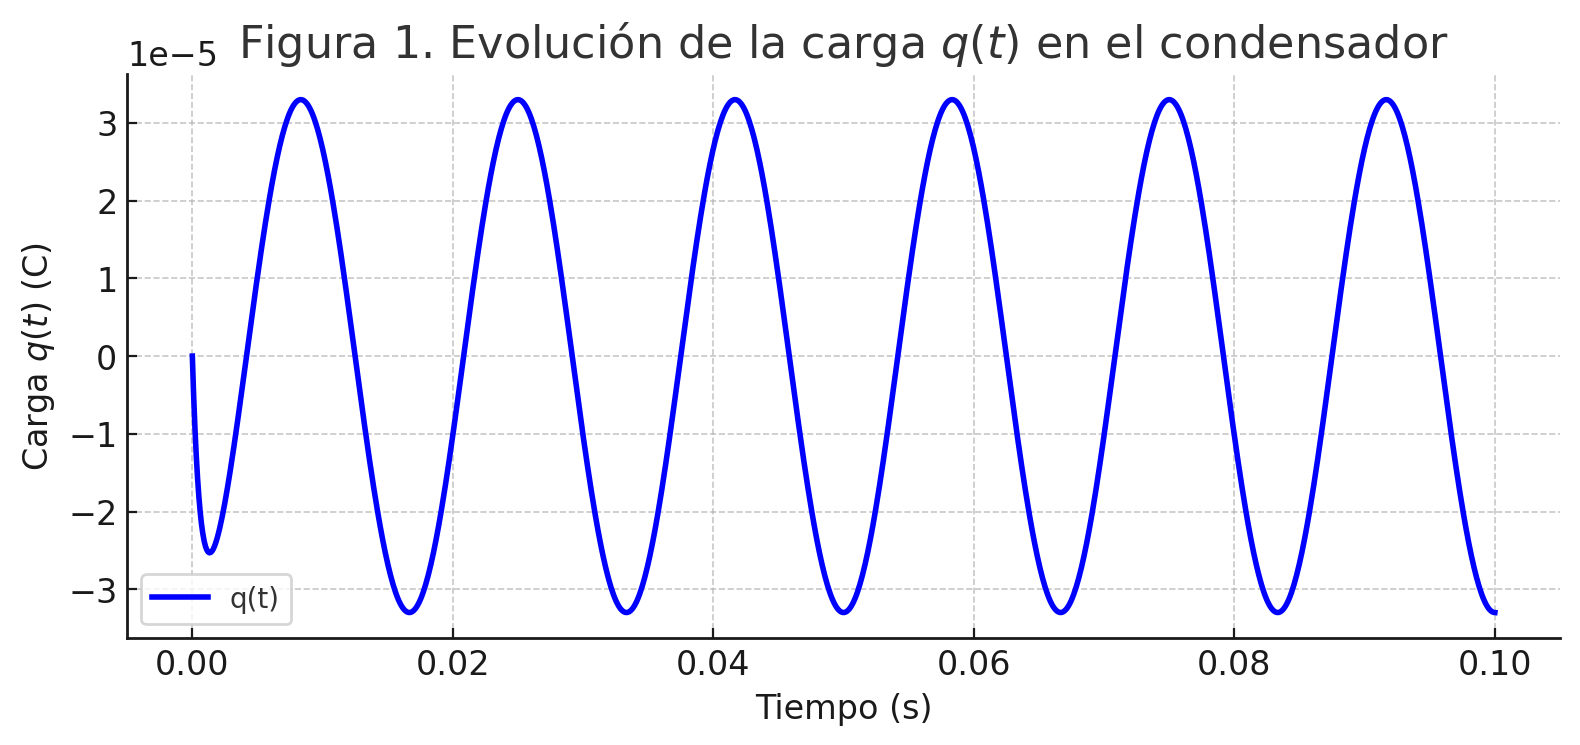
\includegraphics[width=0.8\textwidth]{7.png}
	\caption{Carga del capacitor vs. tiempo}
\end{figure}

\begin{lstlisting}[language=Python, caption={Código Python para simulación de carga}, label={cod:carga}, frame=single, basicstyle=\footnotesize\ttfamily]
import numpy as np
import matplotlib.pyplot as plt

R_bat = 1.2
R_x = 0.1
R_c = 0.3
C = 1000e-6
omega = 2 * np.pi * 60

tau = C * (R_bat + R_x + R_c)

A = 3.2982e-5
B = 5.4679e-8
C_p = -3.2982e-5

t = np.linspace(0, 0.1, 1000)
q_t = A * np.exp(-t / tau) + B * np.sin(omega * t) + C_p * np.cos(omega * t)

plt.figure(figsize=(8, 4))
plt.plot(t, q_t, label='q(t)', color='blue', linewidth=2)
plt.title('Carga en el Capacitor vs. Tiempo')
plt.xlabel('Tiempo (s)')
plt.ylabel('Carga q(t) (C)')
plt.grid(True)
plt.legend()
plt.tight_layout()
plt.show()
\end{lstlisting}

\newpage

\subsection*{Anexo 3: Código y gráfica del análisis espectral de la señal q(t) mediante FFT}
\begin{figure}[H]
	\centering
	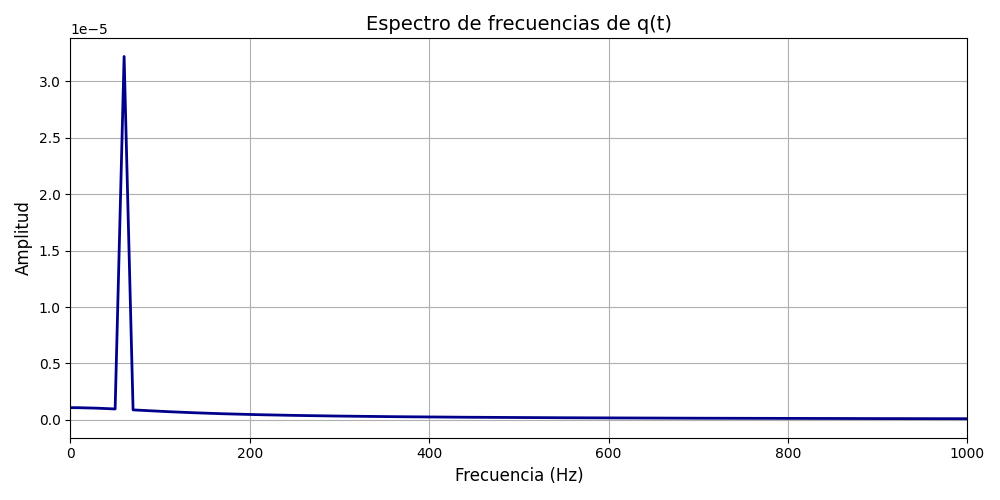
\includegraphics[width=0.8\textwidth]{8.png}
	\caption{Espectro de frecuencias de la señal q(t)}
\end{figure}

\begin{lstlisting}[language=Python, caption={Código Python del análisis espectral}, label={cod:fft}, frame=single, basicstyle=\footnotesize\ttfamily]
import numpy as np
import matplotlib.pyplot as plt
from scipy.fft import fft, fftfreq

tau = 1.6e-3
omega = 2 * np.pi * 60
f_s = 10000
T = 1 / f_s
t = np.arange(0, 0.1, T)

A = 3.2982e-5
B = 5.4679e-8
C = -3.2982e-5


N = len(t)
yf = fft(q_t)
xf = fftfreq(N, T)[:N//2]
amplitud = 2.0 / N * np.abs(yf[0:N//2])

plt.figure(figsize=(10, 5))
plt.plot(xf, amplitud, color='darkblue', linewidth=2)
plt.title('Espectro de frecuencias de q(t)', fontsize=14)
plt.xlabel('Frecuencia (Hz)', fontsize=12)
plt.ylabel('Amplitud', fontsize=12)
plt.grid(True)
plt.xlim(0, 1000)
plt.tight_layout()
plt.show()
\end{lstlisting}


\end{document}